\chapter{Transformada de
Laplace}\label{sec:laplace}\index{transformada de
Laplace}\index{Laplace, transformada de}

La transformada de Laplace \'{e}s part de l'anomenat c\`{a}lcul operacional,
i s'utilitza per convertir equacions diferencials ordin\`{a}ries en
equacions lineals; un cop resoltes aquestes equacions lineals, la
transformada inversa de Laplace ens proporciona la soluci\'{o} de
l'equaci\'{o} diferencial original.

\section{Definicions}\index{transformada de
Laplace!definicions}

\subsection{Transformada de Laplace}

La transformada de Laplace $\mathcal{L}$  converteix una funci\'{o} del
temps $f(t)$, definida per a $t\geq 0$, en una funci\'{o} $F(s)$, on $s$
\'{e}s una variable complexa:
\begin{equation}
    \mathcal{L}\bigl(f(t)\bigr) \equiv F(s) = \int_0^\infty f(t) \,\eu^{-s t} \diff t =
    \lim_{\tau\to\infty} \int_0^\tau f(t) \,\eu^{-s t} \diff t \label{eq:transf_laplace}
\end{equation}

El teorema de l'exist\`{e}ncia de la transformada de Laplace estableix
que si $f(t)$ \'{e}s una funci\'{o} cont\'{\i}nua a trossos, en qualsevol
interval finit contingut en $[0,\infty)$, i satisf\`{a}: $|f(t)| \leq M
\eu^{\alpha t}$ per a qualsevol $t \in [0,\infty)$, llavors la
funci\'{o} $\mathcal{L}\bigl(f(t)\bigr)$ existeix i \'{e}s \'{u}nica per a
qualsevol $s > \alpha$.

\subsection{Transformada inversa de Laplace}

La transformada inversa de Laplace $\mathcal{L}^{-1}$ s'utilitza per
obtenir la funci\'{o} original $f(t)$ a partir de la funci\'{o}
transformada $F(s)$:
\begin{equation}
    \mathcal{L}^{-1}\bigl(F(s)\bigr) \equiv f(t) = \frac{1}{2 \piup \ju }
    \int_{\gamma-\ju \infty}^{\gamma+\ju \infty} F(s)\, \eu^{s t} \diff s
    ,\qquad t\geq 0 \label{eq:transf_inv_laplace}
\end{equation}

On $\gamma$ \'{e}s un cam\'{\i} vertical en el pla complex, escollit de tal
manera que totes les singularitats de la funci\'{o} $F(s)$ quedin a la
seva esquerra.

\subsection{Funci\'{o} gra\'{o} unitari i funci\'{o} impuls}\index{funci\'{o}!gra\'{o}
unitari} \index{funci\'{o}!impuls}\index{funci\'{o}!de
Heaviside}\index{funci\'{o}!delta de Dirac}\index{Heaviside, funci\'{o}
de}\index{Dirac, funci\'{o} delta
de}\index{$\epsilon$@$\varepsilon_\tau(t)$}\index{$\delta_\tau(t)$}

Aquestes dues funcions s\'{o}n de gran import\`{a}ncia en el c\`{a}lcul
operacional. La funci\'{o} gra\'{o} unitari, o funci\'{o} de Heaviside,
$\varepsilon_\tau(t)$ o $\varepsilon(t-\tau)$ en l'instant de temps
$t=\tau$ es defineix com:
\begin{equation}
    \varepsilon_\tau(t) \equiv \varepsilon(t-\tau) = \begin{cases} 1, & t \geq \tau \\ 0, & t < \tau \end{cases}
\end{equation}

La funci\'{o} impuls, o funci\'{o} delta de Dirac, $\delta_\tau(t)$ o
$\delta(t-\tau)$ en l'instant de temps $t=\tau$, es pot definir
mitjan\c{c}ant l'\'{u}s de l\'{\i}mits o d'integrals de variable complexa, per\`{o}
resulta m\'{e}s intu\"{\i}tiu definir-la a partir de les seves propietats: la
funci\'{o} \'{e}s nu{\l.l}a a tot arreu excepte a $t=\tau$, i \'{e}s d'\`{a}rea
unit\`{a}ria:
\begin{subequations}
\begin{align}
    \delta_\tau(t) \equiv \delta(t-\tau) &= 0, \qquad \forall t \neq \tau \\
    \int_{-\infty}^\infty \delta_\tau(t) \diff t &= 1
\end{align}
\end{subequations}

Algunes propietats i relacions de les funcions $\varepsilon_\tau(t)$ i $\delta_\tau(t)$, on $f(t)$ \'{e}s una funci\'{o} qualsevol, s\'{o}n:
\begin{align}
   \frac{\diff}{\diff t} \varepsilon_\tau (t) &= \delta_\tau(t) \\[0.5ex]
   \int_{-\infty}^\infty f(t) \delta_\tau (t) \diff t &= f(\tau) \\[0.5ex]
    \int_a^b \varepsilon_\tau (t) f(t) \diff t &= \varepsilon_\tau(t)
    \int_\tau^b f(t) \diff t, \qquad a\leq\tau\leq b
\end{align}



\section{Propietats}\index{transformada de
Laplace!propietats}

La transformada de Laplace i la seva inversa, verifiquen les
propietats seg\"{u}ents:

\subsection{Linealitat}

Si tenim: $\mathcal{L} \bigl(f_1(t) \bigr) = F_1(s)$ i $\mathcal{L}
\bigl(f_2(t) \bigr) = F_2(s)$, llavors:
\begin{subequations}
\begin{alignat}{2}
    \mathcal{L} \bigl( a_1 f_1(t) + a_2 f_2(t) \bigr) &= a_1 F_1(s) +
    a_2 F_2(s) &\qquad (a_1,a_2 \in \mathbb{R}) \\
    \mathcal{L}^{-1} \bigl( a_1 F_1(s) + a_2 F_2(s) \bigr) &= a_1 f_1(t) +
    a_2 f_2(t) &\qquad (a_1,a_2 \in \mathbb{R})
\end{alignat}
\end{subequations}

\subsection{Canvi d'escala}

Si tenim: $\mathcal{L} \bigl(f(t) \bigr) = F(s)$, llavors:
\begin{subequations}
\begin{alignat}{2}
    \mathcal{L} \bigl( f(a t) \bigr) &= \frac{F(s/a)}{a}
     &\qquad (a \in \mathbb{R}) \\
     \mathcal{L}^{-1} \bigl( F(a s) \bigr) &= \frac{f(t/a)}{a}
     &\qquad (a \in \mathbb{R})
\end{alignat}
\end{subequations}

\subsection{Translaci\'{o}}

Si tenim: $\mathcal{L} \bigl(f(t) \bigr) = F(s)$, llavors:
\begin{subequations}
\begin{alignat}{2}
    \mathcal{L} \bigl( f(t - \tau) \bigr) &= \mathcal{L} \bigl( f(t - \tau)
    \varepsilon_\tau(t) \bigr) = \eu^{-s \tau} F(s) &\qquad (\tau \in \mathbb{R}^+) \\
    \mathcal{L}^{-1} \bigl( \eu^{-s \tau} F(s) \bigr) &=
    f(t-\tau) \varepsilon_\tau(t) &\qquad (\tau \in \mathbb{R}^+)
\end{alignat}
\end{subequations}

\subsection{Esmorte\"{\i}ment}

Si tenim: $\mathcal{L} \bigl(f(t) \bigr) = F(s)$, llavors:
\begin{subequations}
\begin{alignat}{2}
    \mathcal{L} \bigl( \eu^{at} f(t) \bigr) &= F(s-a)
     &\qquad (a \in \mathbb{R})\\
    \mathcal{L}^{-1} \bigl( F(s-a) \bigr) &=\eu^{at} f(t)
     &\qquad (a \in \mathbb{R})
\end{alignat}
\end{subequations}

\subsection{Diferenciaci\'{o}}

Si tenim: $\mathcal{L} \bigl(f(t) \bigr) = F(s)$, on $f(t)$ \'{e}s
diferenciable $n-1$ vegades en l'interval $[0,\infty)$, i compleix
$|f(t)|\leq M\eu^{\alpha t}$ per a qualsevol $t \in [0,\infty)$,
llavors:
\begin{subequations}
\begin{align}
    \mathcal{L} \bigl( f'(t) \bigr) &= s F(s) - f(0)\\
    \mathcal{L} \bigl( f''(t) \bigr) &= s^2 F(s) - s f(0) - f'(0)\\
    \mathcal{L} \bigl( f^{(n)}(t) \bigr) &= s^n F(s) - s^{n-1} f(0) -
    s^{n-2} f'(0) - \cdots - f^{(n-1)}(0)
\end{align}
\end{subequations}

\subsection{Integraci\'{o}}

Si tenim: $\mathcal{L} \bigl(f(t) \bigr) = F(s)$, on $f(t)$ \'{e}s una
funci\'{o} cont\'{\i}nua a trossos, i compleix $|f(t)|\leq M\eu^{\alpha t}$,
llavors:
\begin{align}
    \mathcal{L} \left( \int_0^t f(\tau) \diff \tau \right) = \frac{F(s)}{s}
\end{align}

\subsection{Producte de convoluci\'{o}}\index{producte de convoluci\'{o}}

El producte de convoluci\'{o} de dues funcions $f_1(t)$ i $f_2(t)$ es
defineix com:
\begin{equation}
    f_1(t) * f_2(t) = \int_0^t f_1(\tau) f_2(t-\tau) \diff\tau =
    \int_0^t f_1(t-\tau) f_2(\tau) \diff\tau
\end{equation}

Si tenim: $\mathcal{L} \bigl(f_1(t) \bigr) = F_1(s)$ i $\mathcal{L}
\bigl(f_2(t) \bigr) = F_2(s)$, on $f_1(t)$ i $f_2(t)$ s\'{o}n funcions
cont\'{\i}nues a trossos, i compleixen $|f_1(t)|\leq M_1\eu^{\alpha_1 t}$
i $|f_2(t)|\leq M_2\eu^{\alpha_2 t}$, llavors:
\begin{align}
    \mathcal{L} \bigl( f_1(t) * f_2(t) \bigr) &= F_1(s) F_2(s)\\
    \mathcal{L}^{-1} \bigl( F_1(s) F_2(s) \bigr) &= f_1(t) * f_2(t)
\end{align}

\subsection{Funci\'{o} peri\`{o}dica}

Sigui $f(t)$ una funci\'{o} definida en l'interval $[0,T]$ i nu{\l.l}a
fora d'aquest interval, i sigui $f\ped{P}(t)$ la funci\'{o} peri\`{o}dica de
per\'{\i}ode $T$, que s'origina per repetici\'{o} de la funci\'{o} $f(t)$; si
tenim: $\mathcal{L} \bigl(f(t) \bigr) = F(s)$, llavors:
\begin{equation}
    F\ped{P}(s) = \frac{F(s)}{1-\eu^{-sT}}
\end{equation}

\section{Taules de transformades de Laplace}

Encara que les transformades directa i inversa de Laplace, es poden
obtenir amb les equacions \eqref{eq:transf_laplace} i
\eqref{eq:transf_inv_laplace} respectivament, els c\`{a}lculs
involucrats poden ser for\c{c}a complicats; per aquest motiu \'{e}s usual
disposar de taules que recullen les transformades de Laplace d'un
gran nombre de funcions.

En la Taula \vref{taula:Trans-Laplace-Fun} es pot veure una relaci\'{o} de
transformades de Laplace de les funcions m\'{e}s usuals. Totes les
constants que hi apareixen s\'{o}n valors reals, que tant poden ser
positius com negatius, llevat que s'indiqui el contrari; la variable
$\omega$ que apareix en les funcions trigonom\`{e}triques representa la
velocitat angular ($\omega=2\piup f=2\piup\,/T$).

\index{transformada de Laplace!taula de funcions}
\begin{longtable}{r<{\hspace{3em}}l}
   \caption{\label{taula:Trans-Laplace-Fun} Transformades de Laplace de funcions}\\
   \toprule[1pt]
   $f(t)$ & $F(s) = \mathcal{L} \bigl(f(t) \bigr)$\\
   \midrule
   \endfirsthead
   \caption[]{Transformades de Laplace de funcions (\emph{ve de la p\`{a}gina anterior})} \\
   \toprule[1pt]
   $f(t)$ & $F(s) = \mathcal{L} \bigl(f(t) \bigr)$\\
   \midrule
   \endhead
   \midrule
   \multicolumn{2}{r}{(\emph{continua a la p\`{a}gina seg\"{u}ent})}
   \endfoot
   \endlastfoot
   $\varepsilon_\tau(t), \quad\tau\in\mathbb{R}^+$  & $\dfrac{\eu^{-\tau s}}{s}$\\[2.4ex]
   $\delta_\tau(t), \quad\tau\in\mathbb{R}^+$ & $\eu^{-\tau s}$\\[2.4ex]
   1 & $\dfrac{1}{s}$\\[2.4ex]
   $t$ &   $\dfrac{1}{s^2}$\\[2.4ex]
   $t^n, \quad n\in\mathbb{Z}^+$ &   $\dfrac{n!}{s^{n+1}}$\\[2.4ex]
   $\dfrac{t^{n-1}}{(n-1)!},\quad n\in\mathbb{Z}^+$ & $\dfrac{1}{s^n}$\\[2.4ex]
   $t^a$ & $\dfrac{\Gamma(a+1)}{s^{a+1}}$\\[2.4ex]
   $\dfrac{1}{\sqrt{t}}$ & $\dfrac{\sqrt{\piup}}{\sqrt{s}} $\\[2.4ex]
   $\sqrt{t}$ & $\dfrac{\sqrt{\piup}}{2 s \sqrt{s}}$\\[2.4ex]
   $\dfrac{\eu^{-a t}}{\sqrt{t}}$ & $\dfrac{\sqrt{\piup}}{\sqrt{s+a}}$\\[2.4ex]
   $\eu^{-a t}$ & $\dfrac{1}{s+a}$\\[2.4ex]
   $a^{-b t},\quad a\neq0$ & $\dfrac{1}{s+b\ln a}$\\[2.4ex]
   $1- \eu^{-a t}$ & $\dfrac{a}{s(s+a)}$\\[2.4ex]
   $t \eu^{-a t}$ & $\dfrac{1}{(s+a)^2} $\\[2.4ex]
   $(1-a t)\eu^{-a t}$ & $\dfrac{s}{(s+a)^2} $\\[2.4ex]
   $t^2 \eu^{-a t}$ & $\dfrac{2}{(s+a)^3} $\\[2.4ex]
   $\dfrac{t^{n-1}\eu^{-at}}{(n-1)!},\quad n\in\mathbb{Z}^+$ & $\dfrac{1}{(s+a)^n}$\\[2.4ex]
   $\dfrac{\eu^{-a t}-\eu^{-b t}}{b-a} $ & $\dfrac{1}{(s+a)(s+b)}$\\[2.4ex]
   $\dfrac{\eu^{-t/a}-\eu^{-t/b}}{a-b} $ &  $\dfrac{1}{(a s+1)(b s+1)}$\\[2.4ex]
   $\dfrac{a\eu^{-a t}-b\eu^{-b t}}{a-b} $ &  $\dfrac{s}{(s+a)(s+b)}$\\[2.4ex]
   $\dfrac{a\eu^{-t/b}-b\eu^{-t/a}}{a b(a-b)} $ & $\dfrac{s}{(a s+1)(b s+1)}$\\[2.4ex]
   $\dfrac{\eu^t}{n!}\,\dfrac{\diff^n}{\diff t^n}(t^n e^{-t}),\quad n\in\mathbb{Z}^*$ & $\dfrac{(s-1)^n}{s^{n+1}}$\\[2.4ex]
   $\sin \omega t$ & $\dfrac{\omega}{s^2+\omega^2}$\\[2.4ex]
   $\cos \omega t$ & $\dfrac{s}{s^2+\omega^2}$\\[2.4ex]
   $\sin(\omega t + \varphi)$ & $\dfrac{\omega\cos\varphi+s\sin\varphi}{s^2+\omega^2}$\\[2.4ex]
   $\cos(\omega t + \varphi)$ & $\dfrac{s\cos\varphi-\omega\sin\varphi}{s^2+\omega^2}$\\[2.4ex]
   $t \sin \omega t$ & $\dfrac{2 \omega s}{(s^2+\omega^2)^2}$\\[2.4ex]
   $t \cos \omega t$ & $\dfrac{s^2-\omega^2}{(s^2+\omega^2)^2}$\\[2.4ex]
   $\eu^{-a t} \sin \omega t$ & $\dfrac{\omega}{(s+a)^2+\omega^2}$\\[2.4ex]
   $\eu^{-a t} \cos \omega t$ & $\dfrac{s+a}{(s+a)^2+\omega^2}$\\[2.4ex]
   $\eu^{-a t} \sin (\omega t+\varphi)$ & $\dfrac{\omega\cos\varphi+(s+a)\sin\varphi}{(s+a)^2+\omega^2}$\\[2.4ex]
   $\eu^{-a t} \cos (\omega t+\varphi)$ & $\dfrac{(s+a)\cos\varphi-\omega\sin\varphi}{(s+a)^2+\omega^2}$\\[2.4ex]
   $\sin^2 \omega t$ & $\dfrac{2\omega^2}{s^3+4s\omega^2}$\\[2.4ex]
   $\cos^2 \omega t$ &  $\dfrac{s^2+2\omega^2}{s^3+4s\omega^2}$\\[2.4ex]
   $\dfrac{\sin(2\sqrt{\omega t})}{\sqrt{\omega}}$ & $\dfrac{\sqrt{\piup}\eu^{-\omega/s}}{s\sqrt{s}}$\\[2.4ex]
   $\dfrac{\cos(2\sqrt{\omega t})}{\sqrt{t}}$ & $\dfrac{\sqrt{\piup}\eu^{-\omega/s}}{\sqrt{s}}$\\[2.4ex]
   $\sinh a t$ & $\dfrac{a}{s^2-a^2}$\\[2.4ex]
   $\cosh a t$ & $\dfrac{s}{s^2-a^2}$\\[2.4ex]
   $\sinh^2 a t$ & $\dfrac{2a^2}{s^3-4sa^2}$\\[2.4ex]
   $\cosh^2 a t$ & $\dfrac{s^2-2a^2}{s^3-4sa^2}$\\[2.4ex]
   $t \sinh a t$ & $\dfrac{2 a s}{\left(s^2-a^2\right)^2}$\\[2.4ex]
   $t \cosh a t$ & $\dfrac{s^2+a^2}{\left(s^2-a^2\right)^2}$\\[2.4ex]
   $\eu^{-b t} \sinh a t$ & $ \dfrac{a}{(s+b)^2 - a^2}$\\[2.4ex]
   $\eu^{-b t} \cosh a t$ & $ \dfrac{s+b}{(s+b)^2 - a^2}$\\[3ex]
   $J_\nu(a t),\quad \nu>-1$ & $\dfrac{\left(\sqrt{s^2+a^2}-s\right)^\nu}{a^\nu \sqrt{s^2+a^2}}$\\[2.4ex]
   $I_\nu(a t),\quad \nu>-1$ & $\dfrac{\left(s-\sqrt{s^2-a^2}\right)^\nu}{a^\nu \sqrt{s^2-a^2}}$\\[2.4ex]
   $\dfrac{J_\nu(a t)}{t},\quad \nu>0$ & $\dfrac{\left(\sqrt{s^2+a^2}-s\right)^\nu}{\nu a^\nu}$\\[2.4ex]
   $\dfrac{I_\nu(a t)}{t},\quad \nu>0$ & $\dfrac{\left(s-\sqrt{s^2-a^2}\right)^\nu}{\nu a^\nu}$\\[1.0ex]
   \bottomrule[1pt]
\end{longtable}

\break
En la Taula \vref{taula:Trans-Laplace-Graf} es pot veure una relaci\'{o} de
transformades de Laplace de diverses formes d'ona usuals.

\index{transformada de Laplace!taula de formes d'ona}
\begin{longtable}{cc}
   \caption{\label{taula:Trans-Laplace-Graf} Transformades de Laplace de formes d'ona}\\
   \toprule[1pt]
   $f(t)$ & $F(s) = \mathcal{L} \bigl(f(t) \bigr)$\\
   \midrule
   \endfirsthead
   \caption[]{Transformades de Laplace de formes d'ona (\emph{ve de la p\`{a}gina anterior})} \\
   \toprule[1pt]
   $f(t)$ & $F(s) = \mathcal{L} \bigl(f(t) \bigr)$\\
   \midrule
   \endhead
   \midrule
   \multicolumn{2}{r}{(\emph{continua a la p\`{a}gina seg\"{u}ent})}
   \endfoot
   \endlastfoot
   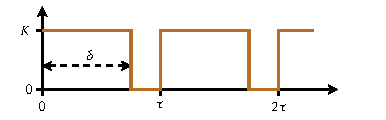
\includegraphics{Imatges/Cap-Laplace-Funcio-1.pdf} & \raisebox{0.8cm}{$K\dfrac{1-\eu^{\delta s}}{s(1-\eu^{-\tau s})}$}\\[2.4ex]
   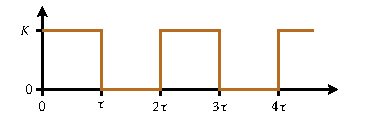
\includegraphics{Imatges/Cap-Laplace-Funcio-2.pdf} & \raisebox{0.8cm}{$\dfrac{K}{s(1+\eu^{-\tau s})}$}\\[2.4ex]
   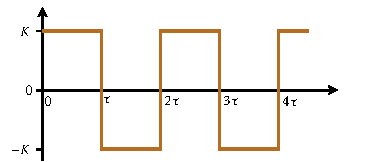
\includegraphics{Imatges/Cap-Laplace-Funcio-3.pdf} & \raisebox{1.2cm}{$K\dfrac{1-\eu^{-\tau s}}{s(1+\eu^{-\tau s})} = \dfrac{K}{s}\tanh\dfrac{\tau s}{2}$}\\[2.4ex]
   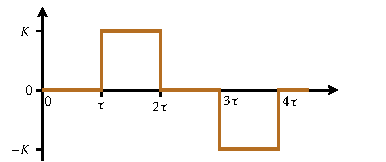
\includegraphics{Imatges/Cap-Laplace-Funcio-4.pdf} & \raisebox{1.2cm}{$K\dfrac{1-\eu^{-\tau s}}{s(\eu^{\tau s}+\eu^{-\tau s})}$}\\[2.4ex]
   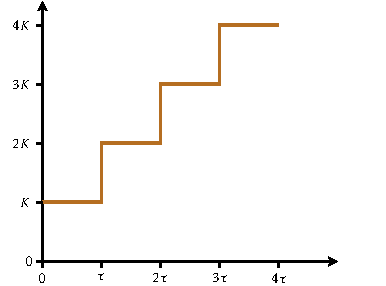
\includegraphics{Imatges/Cap-Laplace-Funcio-5.pdf} & \raisebox{2.5cm}{$\dfrac{K}{s(1-\eu^{-\tau s})} =
   K\dfrac{1+\coth(\frac{\tau s}{2})}{2 s}$}\\[2.4ex]
   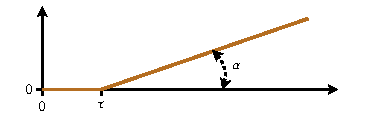
\includegraphics{Imatges/Cap-Laplace-Funcio-6.pdf} & \raisebox{0.8cm}{$\dfrac{\eu^{-\tau s}}{s^2}\tan\alpha$}\\[2.4ex]
   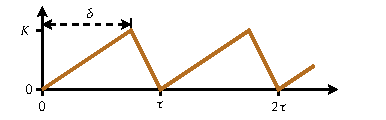
\includegraphics{Imatges/Cap-Laplace-Funcio-7.pdf} & \raisebox{0.8cm}{$K\dfrac{-1+\eu^{-\tau s}+\dfrac{\tau}{\delta}(1-\eu^{-\delta s})}{(\tau-\delta)s^2(1-\eu^{-\tau s})}$}\\[2.4ex]
   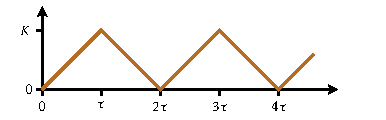
\includegraphics{Imatges/Cap-Laplace-Funcio-8.pdf} & \raisebox{0.8cm}{$K\dfrac{1-\eu^{-\tau s}}{\tau s^2(1+\eu^{-\tau s})} = \dfrac{K}{\tau s^2}\tanh\dfrac{\tau s}{2}$}\\[2.4ex]
   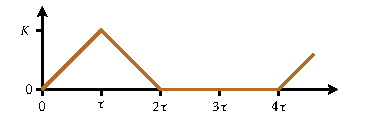
\includegraphics{Imatges/Cap-Laplace-Funcio-9.pdf} & \raisebox{0.8cm}{$K\dfrac{\eu^{-2\tau s}-2\eu^{-\tau s}+1}{\tau s^2(1-\eu^{-4\tau s})}$}\\[2.4ex]
   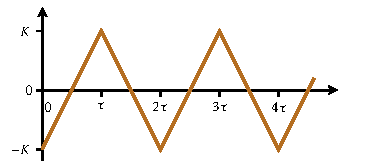
\includegraphics{Imatges/Cap-Laplace-Funcio-10.pdf} & \raisebox{1.2cm}{$2K\dfrac{1-\eu^{-\tau s}}{\tau s^2(1+\eu^{-\tau s})}-\dfrac{K}{s}$}\\[2.4ex]
   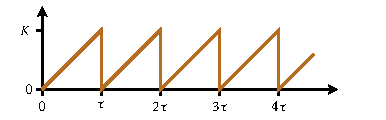
\includegraphics{Imatges/Cap-Laplace-Funcio-11.pdf} & \raisebox{0.8cm}{$\dfrac{K}{\tau s^2}-\dfrac{K\eu^{-\tau s}}{s(1-\eu^{\tau s})}$}\\[2.4ex]
   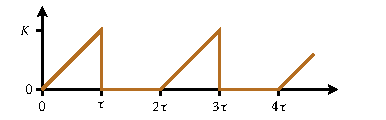
\includegraphics{Imatges/Cap-Laplace-Funcio-12.pdf} & \raisebox{0.8cm}{$K\dfrac{1-(1+\tau s)\eu^{-\tau s}}{\tau s^2(1-\eu^{-2\tau s})}$}\\[2.4ex]
   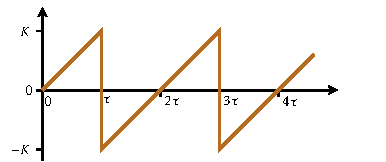
\includegraphics{Imatges/Cap-Laplace-Funcio-13.pdf} & \raisebox{1.2cm}{$\dfrac{K}{\tau s^2}-2K \left(\dfrac{1}{\eu^{-\tau s}-1}-\dfrac{1}{\eu^{2\tau s}-1} \right)$}\\[2.4ex]
   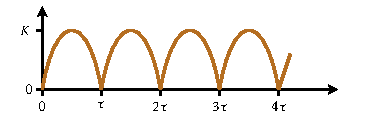
\includegraphics{Imatges/Cap-Laplace-Funcio-14.pdf} & \raisebox{0.8cm}{$K\dfrac{\dfrac{\piup}{\tau}}{s^2+\dfrac{\piup^2}{\tau^2}}\dfrac{(1+\eu^{-\tau s})}{(1-\eu^{-\tau s})}$}\\[2.4ex]
   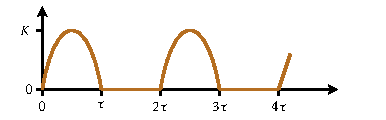
\includegraphics{Imatges/Cap-Laplace-Funcio-15.pdf} & \raisebox{0.8cm}{$K\dfrac{\dfrac{\piup}{\tau}}{s^2+\dfrac{\piup^2}{\tau^2}}\dfrac{1}{(1-\eu^{-\tau s})}$}\\[2.4ex]
    \bottomrule[1pt]
\end{longtable}

\begin{exemple}
    Es tracta de calcular la transformada de Laplace dels dos
    senyals peri\`{o}dics que es mostren a continuaci\'{o}; el primer \'{e}s una
    ona triangular i el segon es la tensi\'{o} sinuso\"{\i}dal que s'obt\'{e} amb un
    rectificador d'ona completa.

\begin{figure}[h]
\centering
    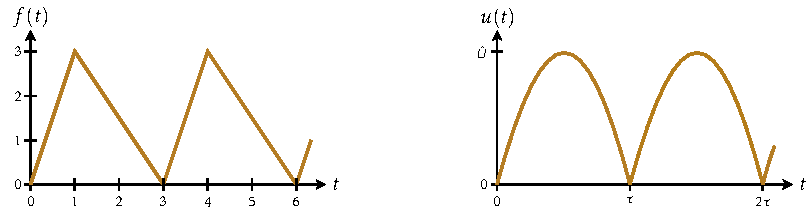
\includegraphics{Imatges/Cap-Laplace-Exemple1.pdf}
\end{figure}

Comencem amb l'ona triangular, estudiant la funci\'{o} $f_1(t)$ definida
entre $t=0$ i $t=3$, i que per repetici\'{o} genera la funci\'{o} $f(t)$; la
seva expressi\'{o} matem\`{a}tica \'{e}s:
\[
    f_1(t) = \begin{cases}
    \phantom{-}0, & t < 0\\
    \phantom{-}3t, & 0<t<1 \\
    -\dfrac{3}{2}t +\dfrac{9}{2}, & 1 < t < 3 \\
    \phantom{-}0, & t > 3 \end{cases}
\]

Amb l'ajut de les funcions gra\'{o} unitari en $t=0$, $t=1$ i $t=3$,
podem definir $f_1(t)$ com:
\[\begin{split}
    f_1(t) &= 3t \bigl(\varepsilon_0(t) - \varepsilon_1(t)\bigr) + \left(-\frac{3}{2}t
    +\frac{9}{2}\right) \bigl(\varepsilon_1(t) -
    \varepsilon_3(t)\bigr) = \\
    &=
    3t\varepsilon_0(t)-3t\varepsilon_1(t)-\frac{3}{2}t \varepsilon_1(t)
    +\frac{3}{2}t \varepsilon_3(t) +\frac{9}{2} \varepsilon_1(t)
    -\frac{9}{2} \varepsilon_3(t) = \\
    &=3t\varepsilon_0(t) -\frac{9}{2}(t-1)\varepsilon_1(t) +
    \frac{3}{2}(t-3)\varepsilon_3(t)
\end{split}\]

Si ens fixem en el 1r terme, veiem en la Taula
\vref{taula:Trans-Laplace-Fun} que la  transformada de $t$ \'{e}s $1/s^2$.
Els termes 2n i 3r tamb\'{e} contenen la funci\'{o} $t$, per\`{o} traslladada
en el temps un valor d'1 i 3 respectivament; per tant, si ens fixem
en la propietat de la translaci\'{o}, veiem que les seves transformades
seran tamb\'{e} $1/s^2$ multiplicades per $\eu^{-s}$ i $\eu^{-3s}$
respectivament. Aix\'{\i} doncs amb aquestes consideracions i fent
servir la propietat de la linealitat tenim:
\[
    F_1(s) = \frac{3}{s^2} - \frac{9 \eu^{-s}}{2 s^2} + \frac{3 \eu^{-3s}}{2
    s^2} =\frac{6-9\eu^{-s}+3\eu^{-3s}}{2s^2}
\]

Finalment, calculem la transformada de la funci\'{o} $f(t)$ original a
partir de la transformada de la funci\'{o} $f_1(t)$, utilitzant la
propietat de les funcions peri\`{o}diques, amb un per\'{\i}ode $T=3$:
\[
    F(s) = \frac{F_1(s)}{1-\eu^{-3s}} = \frac{6-9\eu^{-s}+3\eu^{-3s}}{2s^2(1-\eu^{-3s}) }
\]

Es pot comprovar que aquest resultat \'{e}s el mateix que s'obt\'{e} directament de la taula \vref{taula:Trans-Laplace-Graf}, amb els valors $K=3$, $\delta=1$ i $\tau=3$.

Continuem ara  amb l'ona sinuso\"{\i}dal estudiant la funci\'{o} $u_1(t)$
definida entre $t=0$ i $t=\tau$, i que per repetici\'{o} genera la
funci\'{o} $u(t)$; la seva expressi\'{o} matem\`{a}tica \'{e}s (amb per\'{\i}ode $T=
2\tau$ i velocitat angular $\omega= 2\piup\,/T  = \piup\,/\tau$):
\[
    u_1(t) = \begin{cases} 0, & t < 0\\ \hat{U}\sin\omega t =
    \hat{U}\sin\dfrac{\piup}{\tau}t,  & 0<t<\tau \\ 0, & t > \tau \end{cases}
\]


Amb l'ajut de les funcions gra\'{o} unitari en $t=0$ i $t=\tau$, podem
definir $u_1(t)$ com:
\[
    u_1(t)=\left(\hat{U}\sin\frac{\piup}{\tau}t\right)\bigl(\varepsilon_0(t)-\varepsilon_\tau(t)\bigr)
    =\left(\hat{U}\sin\frac{\piup}{\tau}t\right)\varepsilon_0(t) - \left(\hat{U}\sin\frac{\piup}{\tau}t\right)\varepsilon_\tau(t)
\]

Pel que fa al 2n  terme, si tenim en compte la igualtat
trigonom\`{e}trica: $-\sin \alpha = \sin(\alpha-\frac{T}{2})$, on $T$ \'{e}s
el per\'{\i}ode, tenim:
\[
    u_1(t) = \left(\hat{U}\sin\frac{\piup}{\tau}t\right)\varepsilon_0(t) +
    \left(\hat{U}\sin\left(\frac{\piup}{\tau}t-\tau\right)\right)\varepsilon_\tau(t)
\]

El 2n terme s'ha convertit en una funci\'{o} sinus, com el 1r terme,
per\`{o} traslladada en el temps un valor $\tau$; per tant utilitzant la
transformada de la funci\'{o} sinus que apareix en la Taula
\vref{taula:Trans-Laplace-Fun}, i fent \'{u}s de la propietat de la
translaci\'{o}, tenim:
\[
    F_1(s) = \frac{\hat{U} (\piup\,/\tau)}{s^2 + (\piup\,/\tau)^2} +
    \frac{\hat{U} (\piup\,/\tau)}{s^2 + (\piup\,/\tau)^2} \eu^{-\tau s} =
    \frac{\hat{U} (\piup\,/\tau)}{s^2 + (\piup\,/\tau)^2} \bigl( 1+\eu^{-\tau s}
    \big)
\]

Per acabar, calculem la transformada de la funci\'{o} $u(t)$ original a
partir de la transformada de la funci\'{o} $u_1(t)$, utilitzant la
propietat de les funcions peri\`{o}diques, amb un per\'{\i}ode $T=\tau$:
\[
    F(s) = \frac{F_1(s)}{1-\eu^{-\tau s}} =
    \frac{\hat{U} (\piup\,/\tau) }{s^2 + (\piup\,/\tau)^2}\,\frac{1+\eu^{-\tau s}}{1-\eu^{-\tau
    s}}
\]

Es pot comprovar que aquest resultat \'{e}s el mateix que s'obt\'{e} directament de la taula \vref{taula:Trans-Laplace-Graf}, amb el valor $K=\hat{U}$.
\end{exemple}

\section{An\`{a}lisi de circuits el\`{e}ctrics}\index{transformada de
Laplace!an\`{a}lisi de circuits el\`{e}ctrics}\index{an\`{a}lisi de circuits
el\`{e}ctrics}

La transformada de Laplace \'{e}s \'{u}til en la resoluci\'{o} de circuits
el\`{e}ctrics, quan a m\'{e}s del r\`{e}gim permanent es vol con\`{e}ixer
l'evoluci\'{o} transit\`{o}ria pr\`{e}via que tenen les tensions i els corrents.

Mitjan\c{c}ant la transformada de Laplace, les equacions diferencials
que relaciones tensions i corrents, es converteixen en equacions
lineals de m\'{e}s f\`{a}cil resoluci\'{o}. Un cop calculats els valors de
tensions i corrents en el domini operacional, utilitzem la
transformada inversa de Laplace per obtenir els valors d'aquestes
tensions i corrents en el domini temporal.

Per resoldre aquests tipus de circuits, cal con\`{e}ixer-ne les
condicions inicials, \'{e}s a dir, els corrents de les induct\`{a}ncies i
les tensions dels condensadors. Un circuit el\`{e}ctric es diu que est\`{a}
relaxat, quan en l'instant inicial tots els condensadors estan
descarregats i no circula corrent per cap induct\`{a}ncia.

A tall d'exemple, tenim el circuit de la Figura
\vref{pic:transf-Laplace}, on en l'instant inicial $t=0$ circula un
corrent $i_0$ i el condensador $C$ est\`{a} carregat a una tensi\'{o} $u_0$.
\begin{figure}[h]
\centering
    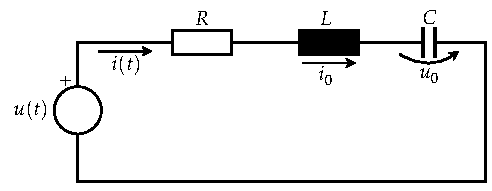
\includegraphics{Imatges/Cap-Laplace-Circuit-RLC.pdf}
\caption{An\`{a}lisi de circuits mitjan\c{c}ant la transformada de Laplace}
\label{pic:transf-Laplace}
\end{figure}

Escrivim en primer lloc  la relaci\'{o} entre $u(t)$ i $i(t)$, a partir
de les relacions individuals entre tensi\'{o} i corrent per a cada
component del circuit, les quals s'han exposat en la Secci\'{o}
\vref{sec:comp_elem}:
\begin{equation}
    u(t) = R i(t) + L \frac{\diff i(t)}{\diff t} + u_0 + \frac{1}{C}
    \int_0^t i(t) \diff t
\end{equation}

Transformem a continuaci\'{o} aquesta equaci\'{o} en una altra en el domini
operacional, essent $\mathcal{L}\bigl(u(t)\bigr) = U(s)$,
$\mathcal{L}\bigl(i(t)\bigr) = I(s)$ i $\mathcal{L}\bigl(u_0\bigr) =
u_0/s$, i aplicant les propietats de la diferenciaci\'{o} i de la
integraci\'{o} a $i(t)$:
\begin{equation}\begin{split}
    U(s) &= R I(s) + L(s I(s) -i_0) + \frac{u_0}{s} + \frac{I(s)}{s
    C} =\\[1ex]
    &= \left( R + s L +\frac{1}{s C}\right)I(s) + \frac{u_0}{s} - L i_0
\end{split}\end{equation}

De fet, aquesta equaci\'{o} la podr\'{\i}em haver escrit directament a
partir de les relacions entre les tensions i els corrents en el
domini operacional per a cada  component del circuit, les quals
s'han exposat tamb\'{e} en la Secci\'{o} \vref{sec:comp_elem}.

Per tant, essent $u(t)$  una funci\'{o} determinada (sinuso\"{\i}dal, impuls,
gra\'{o}, etc...), podem obtenir $U(s)$ i calcular $I(s)$ mitjan\c{c}ant:
\begin{equation}
    I(s) = \frac{U(s)-\dfrac{u_0}{s} + L i_0}{R + s L
    +\dfrac{1}{s C}}\label{eq:i-Laplace}
\end{equation}

Finalment, obtenim el corrent en el domini temporal: $i(t) =
\mathcal{L}^{-1}\bigl(I(s)\bigr)$.

\begin{exemple}

A partir del circuit de la Figura \vref{pic:transf-Laplace}, amb
$L=0$, $i_0=0$ i $u_0=0$, es tracta de calcular el corrent $i(t)$,
essent $u(t)=U$ (valor constant).

Comencem per escriure l'equaci\'{o} \eqref{eq:i-Laplace} en el nostre
cas particular, tenint en compte que $\mathcal{L}(U) = U/s$
\[
    I(s) = \frac{U}{s\left(R + \dfrac{1}{s C}\right)} = \frac{C U}{1 + s R C}
\]

A continuaci\'{o}, dividim numerador i denominador per $R C$ per tal
d'obtenir una expressi\'{o} que es trobi en la Taula
\vref{taula:Trans-Laplace-Fun}:
\[
    I(s) = \frac{\dfrac{U}{R}}{\dfrac{1}{R C} + s}
\]

La transformada inversa de Laplace de $I(s)$, ens d\'{o}na:
\[
    i(t) = \frac{U}{R} \eu^{-\frac{1}{R C}t}
\]

\end{exemple}

\section{Fraccions parcials}\index{fraccions parcials}
\index{transformada de Laplace!fraccions parcials}

En l'exemple anterior, la funci\'{o} de variable $s$ que hem hagut de
buscar en la Taula \vref{taula:Trans-Laplace-Fun} era for\c{c}a simple, i
per tant la seva transformada inversa s'ha obtingut de forma
immediata. El m\'{e}s usual, no obstant, \'{e}s tenir funcions racionals
(quocient de dos polinomis) de grau elevat; en aquest cas cal
descompondre aquesta funci\'{o} racional en suma de funcions parcials de
grau menor.

S'exposa a continuaci\'{o} la teoria de la descomposici\'{o} en fraccions
parcials:

Sigui una funci\'{o} racional $\frac{P(x)}{Q(x)}$, on el grau de $P(x)$
\'{e}s menor que el de $Q(x)$, i el coeficient del terme de grau m\'{e}s
elevat de $Q(x)$ val 1. Si $Q(x)$ t\'{e} $n$ arrels reals sense
multiplicitat: $a_1,\ldots,a_n$, $k$ arrels reals: $b_1,\ldots,b_k$
cadascuna amb la seva multiplicitat: $m_1,\ldots,m_k$, i $l$ arrels
complexes conjugades sense multiplicitat: $c_1\pm
\ju\,d_1,\ldots,c_l\pm \ju\,d_l$, aquest polinomi es pot escriure
com el producte seg\"{u}ent:
\begin{equation}
    Q(x)= (x-a_1) \cdots (x-a_n)(x-b_1)^{m_1} \cdots (x-b_k)^{m_k}
    \bigl((x-c_1)^2+d_1^2\bigr)\cdots\bigl((x-c_l)^2+d_l^2\bigr)
\end{equation}

Les arrels $a_i$ s\'{o}n, de fet, un cas particular de les arrels $b_i$,
amb multiplicitat 1.

A parir de les arrels de $Q(x)$, la funci\'{o}  racional
$\frac{P(x)}{Q(x)}$ es pot expressar com:
\begin{equation}\begin{split}
    \frac{P(x)}{Q(x)} &= \frac{A_1}{x-a_1} + \frac{A_2}{x-a_2}
    + \cdots + \frac{A_n}{x-a_n} +{} \\[1.5ex]
   &+ \frac{B_{1,1}}{(x-b_1)^{m_1}} + \frac{B_{1,2}}{(x-b_1)^{m_1-1}}
   + \frac{B_{1,3}}{(x-b_1)^{m_1-2}} + \cdots +
   \frac{B_{1,m_1}}{x-b_1}+{} \\[1.5ex]
&+ \frac{B_{2,1}}{(x-b_2)^{m_2}} + \frac{B_{2,2}}{(x-b_2)^{m_2-1}}
   + \frac{B_{2,3}}{(x-b_2)^{m_2-2}} + \cdots  +
   \frac{B_{2,m_2}}{x-b_2} +{}\\[1.5ex]
   &+ \cdots +\\[1ex]
&+ \frac{B_{k,1}}{(x-b_k)^{m_k}} + \frac{B_{k,2}}{(x-b_k)^{m_k-1}}
   + \frac{B_{k,3}}{(x-b_k)^{m_k-2}} + \cdots +
   \frac{B_{k,m_k}}{x-b_k}+{}\\[1.5ex]
&+ \frac{C_1(x-c_1)+D_1 d_1}{(x-c_1)^2+d_1^2}+ \frac{C_2(x-c_2)+D_2
d_2}{(x-c_2)^2+d_2^2} +  \cdots +\frac{C_l(x-c_l)+D_l d_l}{(x-c_l)^2+d_l^2}\\[1.5ex]
\end{split}\end{equation}

Els coeficients $A_i$, $B_{i,j}$, $C_i$ i $D_i$, es calculen a
partir de les equacions seg\"{u}ents:
\begin{subequations}
\begin{alignat}{2}
     &A_i = \left. (x-a_i)\frac{P(x)}{Q(x)} \right|_{x=a_i}
     &\qquad i=1,\ldots,n\\[1.5ex]
     &B_{i,j} = \left. (x-b_i)^{m_i} \frac{P(x)}{Q(x)}\right|_{x=b_i}
     &\qquad i=1,\ldots,k; \quad j=1 \\[1.5ex]
    &B_{i,j} = \left. \frac{1}{(j-1)!} \; \frac{\diff^{j-1}}{\diff
    x^{j-1}} \left[ (x-b_i)^{m_i} \frac{P(x)}{Q(x)}\right]\right|_{x=b_i}
     &\qquad i=1,\ldots,k; \quad j=2,\ldots,m_i\\[1.5ex]
   &D_i+\ju\, C_i  =  \left.\frac{1}{d_i} \bigl((x-c_i)^2+d_i^2\bigr) \frac{P(x)}{Q(x)}
    \right|_{x=c_i+\ju\,d_i} &\qquad i=1,\ldots,l
\end{alignat}
\end{subequations}

\begin{exemple}

El circuit de la figura seg\"{u}ent es troba en r\`{e}gim estacionari. En
l'instant $t=0$ s'obre l'interruptor M; es tracta de trobar
l'evoluci\'{o} del corrent $i\ped{L}(t)$, que circula per la induct\`{a}ncia
$L$, a partir d'aquest instant.

\begin{figure}[h]
    \centering
    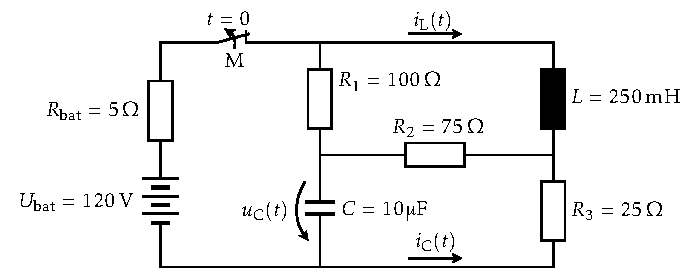
\includegraphics{Imatges/Cap-Laplace-Exemple3-Circuit.pdf}
\end{figure}

 Donat que abans d'obrir l'interruptor M, el circuit ha arribat al
 r\`{e}gim estacionari, el condensador $C$ estar\`{a} totalment carregat  i
 presentar\`{a} una imped\`{a}ncia infinita al corrent continu originat per la
 bateria, i la induct\`{a}ncia $L$ hi presentar\`{a} una imped\`{a}ncia nu{\l.l}a;
 per tant, en l'instant $t=0\unit{s}$, els valors inicials $i\ped{L}(0)$ i
 $u\ped{C}(0)$ s\'{o}n:
 \begin{align*}
    i\ped{L}(0) &= \frac{U\ped{bat}}{R\ped{bat} + R_3} = \frac{120\unit{V}}
    {5\unit{\ohm} + 25\unit{\ohm}} = 4\unit{A} \\[0.5ex]
    u\ped{C}(0) &= i\ped{L}(0) R_3 = 4\unit{A}\cdot 25\unit{\ohm} = 100\unit{V}
 \end{align*}

Un cop obrim l'interruptor M, la bateria i la seva resist\`{e}ncia
queden desconnectades de les dues malles de la part dreta del circuit; si apliquem la llei de les tensions de Kirchhoff  a aquestes
dues malles, utilitzant les variables $I\ped{L}(s)$, $U\ped{C}(s)$ i
$I\ped{C}(s)$, tenim:
\begin{align*}
    R_1 I\ped{L}(s) + s L I\ped{L}(s) - L i\ped{L}(0) + R_2
    \bigl(I\ped{L}(s) + I\ped{C}(s)\bigr) &=0 \\[0.5ex]
    U\ped{C}(s) + R_3 I\ped{C}(s) + R_2 \bigl(I\ped{L}(s) + I\ped{C}(s)\bigr) &=0
\end{align*}

La relaci\'{o} entre $U\ped{C}(s)$ i $I\ped{C}(s)$ \'{e}s:
\begin{equation*}
    U\ped{C}(s) = \frac{I\ped{C}(s)}{s C} + \frac{u\ped{C}(0)}{s}
    \quad\rightarrow\quad I\ped{C}(s) = s C U\ped{C}(s) - C u\ped{C}(0)
\end{equation*}

Si substitu\"{\i}m aquest valor de $I\ped{C}(s)$ en les dues equacions
inicials, i reordenem els seus termes, tenim:
\begin{align*}
    R_1 I\ped{L}(s) + s L I\ped{L}(s)  + R_2
    I\ped{L}(s) + s C R_2 U\ped{C}(s) &= L i\ped{L}(0) + C R_2 u\ped{C}(0)\\[0.5ex]
    U\ped{C}(s) + s C R_3 U\ped{C}(s) + R_2 I\ped{L}(s) + s C R_2 U\ped{C}(s)
    &= C R_3 u\ped{C}(0) + C R_2 u\ped{C}(0)
\end{align*}

Agrupem a continuaci\'{o} els termes comuns i substitu\"{\i}m $u\ped{C}(0)$ i
$i\ped{L}(0)$ pels seus valor num\`{e}rics:
\begin{align*}
    (R_1 + s L + R_2) I\ped{L}(s) + s C R_2 U\ped{C}(s) &= 4 L  + 100 C R_2\\[0.5ex]
    R_2 I\ped{L}(s) + (1 +s C R_3 + s C R_2) U\ped{C}(s) &= 100 C R_3  + 100 C R_2
\end{align*}

A\"{\i}llem ara $U\ped{C}(s)$ en la primera equaci\'{o}:
\[
    U\ped{C}(s) = \frac{4 L  + 100 C R_2 -(R_1 + s L + R_2) I\ped{L}(s)}{s C R_2}
\]

Substitu\"{\i}m tot seguit aquest valor en la segona equaci\'{o}, i a\"{\i}llem
$I\ped{L}(s)$:
\begin{gather*}
   R_2 I\ped{L}(s) + (1 + s C R_3 + s C R_2) \frac{4 L  + 100 C R_2 - (R_1 + s L + R_2)I\ped{L}(s)}{s C R_2} = 100 C R_3  + 100 C R_2 \\[1.5ex]
   \begin{split} &\left( R_2 - \frac{(1 +s C R_3 + s C R_2)(R_1 + s L + R_2)}{s C R_2} \right) I\ped{L}(s)
   = \\[1ex] &= 100 C (R_3  + R_2) - \frac{(1 +s C R_3 + s C R_2)(4 L  + 100 C R_2)}{s C
   R_2}\end{split}\\[1.5ex]
I\ped{L}(s) = \frac{100 s C^2 R_2(R_3  + R_2)- (1 +s C R_3 + s C
R_2)(4 L  + 100 C R_2)}{s C R_2^2  -(1 +s C R_3 + s C R_2)(R_1 + s L
+ R_2)}
\end{gather*}

Si donem valors num\`{e}rics a $R_1$, $R_2$, $R_3$, $L$ i $C$, i
realitzem tots els productes i les  simplificacions oportunes,
tenim:
\[
I\ped{L}(s) = \frac{4 s+ 4300}{s^2 +1475 s + 700000}
\]

Hem de descompondre a continuaci\'{o} aquesta funci\'{o} racional en
funcions parcials; comencem doncs per calcular les arrels del
polinomi del denominador:
\[
s^2 +1475 s + 700000 = 0 \quad\rightarrow\quad s= -\frac{1475}{2}
\pm \ju\,\frac{75\sqrt{111}}{2}
\]

A partir d'aquests valors, la  funci\'{o} racional es pot escriure com:
\[
    I\ped{L}(s) =
    \frac{4 s+ 4300}{s^2 +1475 s + 700000} =
    \frac{C\left(s+\dfrac{1475}{2}\right)+D\dfrac{75\sqrt{111}}{2}}
    {\left(s+\dfrac{1475}{2}\right)^2+\left(\dfrac{75\sqrt{111}}{2}\right)^2}
\]

Les constants $C$ i $D$ valen:
\[
D + \ju\,C = \left.\frac{2}{75\sqrt{111}}(4 s
+4300)\right|_{s=-\frac{1475}{2} + \ju\,\frac{75\sqrt{111}}{2}}=
12\sqrt{\frac{3}{37}} +\ju\,4
\]

Aix\'{\i} doncs, amb $C=4$ i $D=12\sqrt{\frac{3}{37}}$, podem expressar
el corrent $I\ped{L}(s)$ com:
\[
    I\ped{L}(s) = 4\frac{s+\dfrac{1475}{2}}
    {\left(s+\dfrac{1475}{2}\right)^2+\left(\dfrac{75\sqrt{111}}{2}\right)^2}
    + 12\sqrt{\frac{3}{37}}\frac{\dfrac{75\sqrt{111}}{2}}
    {\left(s+\dfrac{1475}{2}\right)^2+\left(\dfrac{75\sqrt{111}}{2}\right)^2}
\]


 Si ens fixem ara en la Taula \vref{taula:Trans-Laplace-Fun},
veiem que la transformada inversa de Laplace del primer terme de
$I\ped{L}(s)$, es pot identificar amb una funci\'{o} del tipus
$\eu^{-at}\cos\omega t$, i la del segon amb una funci\'{o} del tipus
$\eu^{-at}\sin\omega t$, amb $a=\frac{1475}{2}$ i
$\omega=\frac{75\sqrt{111}}{2}$.

Per tant, l'expressi\'{o} temporal del corrent $i\ped{L}(t)$ \'{e}s:
\[\begin{split}
    i\ped{L}(t) &= 4\, \eu^{-\frac{1475}{2}t} \cos \frac{75\sqrt{111}}{2} t +
    12\sqrt{\frac{3}{37}}\, \eu^{-\frac{1475}{2}t} \sin
    \frac{75\sqrt{111}}{2}t = \\[1ex] &= \eu^{-\frac{1475}{2}t} \left( 4
    \cos \frac{75\sqrt{111}}{2} t + 12\sqrt{\frac{3}{37}}\sin
    \frac{75\sqrt{111}}{2}t\right)
\end{split}\]

Finalment, si utilitzem la igualtat trigonom\`{e}trica
\eqref{eq:AcosBsin}, tenim:
\[
i\ped{L}(t) = \frac{32}{\sqrt{37}}\,\eu^{-\frac{1475}{2}t}
\cos\left(\frac{75\sqrt{111}}{2} t - \arctan
\sqrt{\frac{27}{37}}\right)
\]

Si en aquesta equaci\'{o}, fem $t=0\unit{s}$, tenim:
\[
    i\ped{L}(0) = \frac{32}{\sqrt{37}} \cos\left( - \arctan
\sqrt{\frac{27}{37}}\right) = 4 \unit{A}
\]

Es comprova que aquest valor compleix amb la condici\'{o} inicial del
corrent $i\ped{L}(t)$ que hem calculat a l'inici d'aquest exemple.

Representem a continuaci\'{o} la gr\`{a}fica d'aquesta funci\'{o}:
\begin{figure}[h]
\centering
  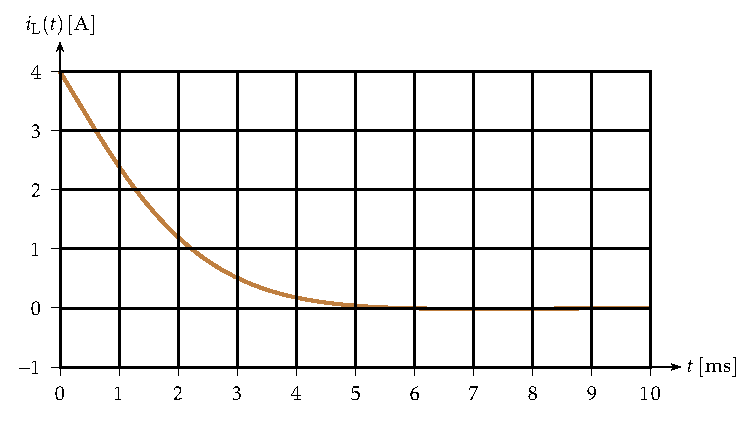
\includegraphics{Imatges/Cap-Laplace-Exemple3-Corrent.pdf}
\end{figure}

\end{exemple}


\begin{exemple}
El circuit de la figura seg\"{u}ent est\`{a} relaxat. En l'instant $t=0$ es
tanca l'interruptor M; es tracta de trobar l'evoluci\'{o} de la tensi\'{o}
$u\ped{C}(t)$, a partir d'aquest instant.
\begin{figure}[h]
\centering
    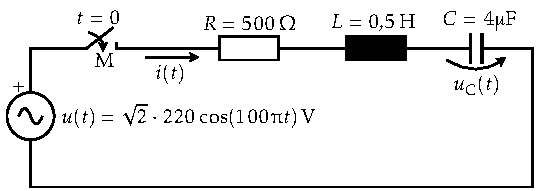
\includegraphics{Imatges/Cap-Laplace-Exemple4-Circuit.pdf}
\end{figure}


La transformada de Laplace de la tensi\'{o} $u(t)$ \'{e}s:
\[
    U(s) = \sqrt{2}\cdot 220 \frac{s}{s^2 + (100\piup)^2}
\]

\break
Un cop tancat l'interruptor M, la relaci\'{o} entre $u\ped{c}(t)$ i
$u(t)$ en el domini operacional, tenint en compte que totes les
condicions inicials s\'{o}n nu{\l.l}es, \'{e}s:
\[
    U\ped{C}(s) = \frac{\dfrac{1}{sC}}{R+ sL +\dfrac{1}{sC}} U(s)=
    \frac{\dfrac{1}{CL}}{s^2 + \dfrac{R}{L}s +\dfrac{1}{CL}} U(s)
\]

Substituint $U(s)$ per la seva expressi\'{o}, i donant valors num\`{e}rics a
$R$, $L$ i $C$, tenim:
\[
    U\ped{C}(s) = \frac{\sqrt{2}\cdot 110\cdot 10^6 s}{(s^2 + 1000 s + 500000)(s^2 + (100\piup)^2)}
\]

Calculem a continuaci\'{o}, les arrels dels dos polinomis  del
denominador d'aquesta funci\'{o} racional:
\begin{align*}
    s^2 + 1000 s + 500000 &= 0 \quad\rightarrow\quad s = -500
    \pm\ju\,500 \\[0.5ex]
    s^2 + (100\piup)^2 &= 0 \quad\rightarrow\quad s = \pm\ju\,100\piup
\end{align*}

Aix\'{\i} doncs, l'esmentada funci\'{o} racional es pot escriure com:
\[\begin{split}
U\ped{C}(s) &= \frac{\sqrt{2}\cdot 110\cdot 10^6 s}{(s^2 + 1000 s +
500000)(s^2 + (100\piup)^2)}  = \\[2ex] &= \frac{C_1 (s+500) + D_1
500}{(s+500)^2+500^2} + \frac{C_2 s + D_2 100 \piup}{s^2 +(100\piup)^2}
\end{split}\]


Les constants $C_1$, $D_1$,  $C_2$ i $D_2$ valen:
\begin{alignat*}{2}
    D_1 + \ju\,C_1 &= \left.\frac{1}{500}\cdot \frac{\sqrt{2}\cdot 110\cdot 10^6 s}
    {s^2 +(100\piup)^2}\right|_{s=-500+\ju\,500} &&=-358{,}57 -\ju\,
    240{,}35\\[2ex]
    D_2 + \ju\,C_2 &= \left.\frac{1}{100\piup}\cdot\frac{\sqrt{2}\cdot 110\cdot 10^6 s}
    {s^2 + 1000 s + 500000}\right|_{s=\ju\,100\piup} &&= 188{,}16 + \ju\,240{,}35
\end{alignat*}

A partir d'aquests valors, i utilitzant la Taula
\vref{taula:Trans-Laplace-Fun}, obtenim l'expressi\'{o} temporal de la
tensi\'{o} en el condensador $u\ped{C}(t)$:
\[
    u\ped{C}(t) = \eu^{-500t} (-240{,}35 \cos 500 t - 358{,}57 \sin 500
    t) + 240{,}35 \cos (100\piup t) + 188{,}16 \sin( 100\piup
    t)
\]

Utilitzant la igualtat trigonom\`{e}trica \eqref{eq:AcosBsin} obtenim finalment:
\[
    u\ped{C}(t)= 431{,}67 \eu^{-500t} \cos(500 t +2{,}1613) + 305{,}24 \cos (100\piup t - 0{,}6642)
\]

\break
Representem a continuaci\'{o} la gr\`{a}fica d'aquesta
funci\'{o}:

\begin{figure}[h]
\centering
  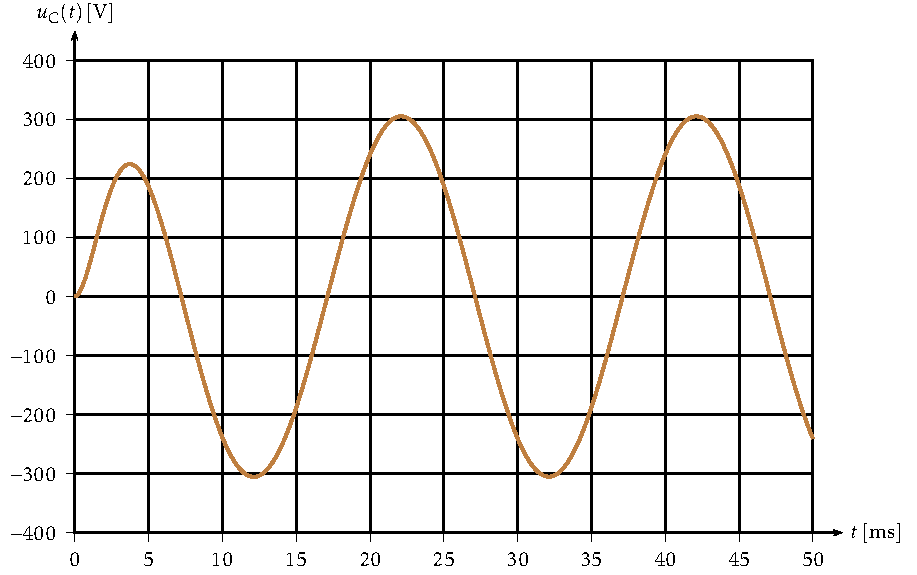
\includegraphics{Imatges/Cap-Laplace-Exemple4-Tensio.pdf}
\end{figure}

\end{exemple}
